\documentclass[a4paper, 12pt]{book}
\usepackage{graphicx}
\usepackage[french]{babel}
\usepackage{caption}
\usepackage[utf8]{inputenc}
\usepackage[T1]{fontenc}
\usepackage{multirow}
\usepackage{listings}
\usepackage{float}
\usepackage{url}
\usepackage[french]{algorithm}
\usepackage{style/myalgorithm}
\usepackage{amsmath,amsfonts,amssymb}
\newcommand{\fBm}{\emph{fBm}~}
\newcommand{\etal}{\emph{et al.}~}
\newcommand{\glAd}{\emph{GL4D}~}
\newcommand{\apiopengl}{API OpenGL\textsuperscript{\textregistered}~}
\newcommand{\opengl}{OpenGL\textsuperscript{\textregistered}~}
\newcommand{\opengles}{OpenGL\textsuperscript{\textregistered}ES~}
\newcommand{\clang}{langage \texttt{C}}
\newcommand{\codesource}{\textsc{Code source}~}
\floatstyle{ruled}
\newfloat{programslist}{htbp}{locs}
\newcommand{\listofprograms}{\listof{programslist}{Liste des codes source}}
\newcounter{program}[subsection]
\renewcommand{\theprogram}{\arabic{chapter}.\arabic{program}}

\newenvironment{program}[1]{
  \if\relax\detokenize{#1}\relax
  \gdef\mycaption{\relax}
  \else
  \gdef\mycaption{#1}
  \fi
  \refstepcounter{program}
  \addcontentsline{locs}{section}{#1}
  \footnotesize
}{
  \begin{description}
    \item[\codesource \theprogram]--~\mycaption
  \end{description}
}

\begin{document}
\begin{titlepage}
  \begin{center}
    \begin{tabular*}{\textwidth}{l@{\extracolsep{\fill}}r}
      
\includegraphics[height=1.5cm]{images/m2ise.png}
    \end{tabular*}
    \small 
    \rule{\textwidth}{.5pt}~\\
    \large 
    \textsc{Université Paris 8 - Vincennes à Saint-Denis}\vspace{0.5cm}\\
    \textbf{Master Informatique des Systèmes Embarqués}\vspace{3.0cm}\\
    \Large
    \textbf{Memoire de projet tuteuré}\vspace{1.5cm}\\
    \large
    \textbf{Fakhri \textsc{YAHIAOUI} - Roman \textsc{BOURSIER}}\vspace{1.5cm}\\
    Date de soutenance : le 09/06/2020\vspace{1.75cm}\\
  \end{center}\vspace{1.5cm}~\\
  \begin{tabular}{ll}
    \hspace{-0.45cm}Tuteur -- Université~:~&~Farès \textsc{BELHADJ}\\
  \end{tabular}
\end{titlepage}
\frontmatter
\chapter*{Résumé}
\markboth{\sc Résumé}{}
\addcontentsline{toc}{chapter}{Résumé} 

A faire en dernier ...


\chapter*{Remerciements}
\markboth{\sc Remerciements}{}
\addcontentsline{toc}{chapter}{Remerciements} 

Idem ...

%% Table des matières
\tableofcontents

\mainmatter
\chapter*{Introduction}
\markboth{\sc Introduction}{}
\addcontentsline{toc}{chapter}{Introduction}

\section{Contexte}
Dans le cadre de notre projet de fin d'étude, nous souhaitons utiliser un modèle d’apprentissage automatique du type Deep Learning, afin de produire un moteur de rendu capable d’adopter une stylisation « type » telle que la peinture chinoise. Dans un premier temps, il s’agira de proposer un modèle d’abstraction des peintures sélectionnées comme base d’apprentissage et d’utiliser le couple « peinture originale » / « abstraction » pour l’entraînement. Par la suite, un moteur de rendu d’abstractions sera connecté au réseau profond qui produira une peinture sur la base de l’abstraction.

Le modèle généré devra d'une part adopter la stylisation retenue mais aussi interpréter l'abstraction d'origine.

\section{Problématique}

De nombreux travaux autour de la "translation d'image à image" \cite{DBLP:journals/corr/IsolaZZE16} permettent déjà d'obtenir de bons résultats.

La figure n°1 montre qu'il est possible de générer un paysage à partir de quelques lignes. Cependant, nous sommes confronté à un problème avec la figure n°2.

\begin{center}
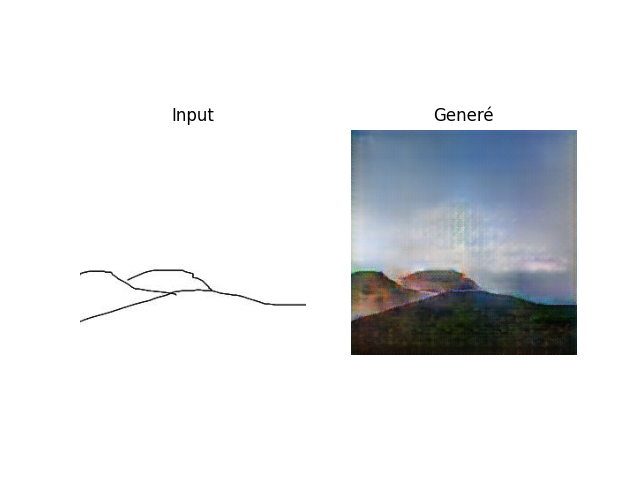
\includegraphics[scale=0.5]{images/pix2pix-t1.png}
\captionof{figure}{Nous avons testé pix2pix sur un dataset composé de photos de paysages que nous avons labellisées en appliquant un filtre canny. Le résultat présenté montre le rendu une fois l'apprentissage terminé, avec un dessin fait à main levée en entrée}
\label{fig1}
\end{center}

\begin{center}
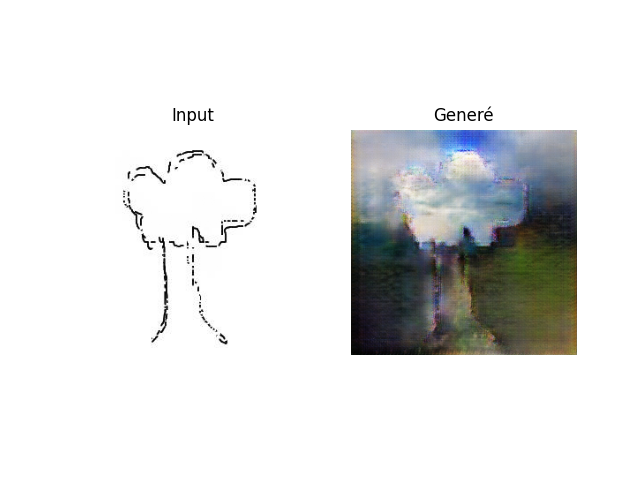
\includegraphics[scale=0.7]{images/pix2pix-fail.png}
\captionof{figure}{Utilisation de pix2pix avec une abstraction d'arbre}
\label{fig1}
\end{center}


Comme évoqué dans \cite{DBLP:journals/corr/abs-1805-00247} ce type de modèle se basent sur une corrélation d'une image à l'autre, et relève d'un apprentissage supervisé. Cependant la distance entre une abstraction et une peinture est dans notre cas trop grande, ce qui nous indique peut-être que ce problème relève d'une part de "non supervisé". 


Nous avons demandé à un plusieurs personnes de dessiner schématiquement un paysage composé de montagnes et d'arbres éléments courants dans une peinture de paysages chinoise: 
\paragraph{}
\includegraphics[width=0.25\linewidth]{images/croquis_1.jpg}
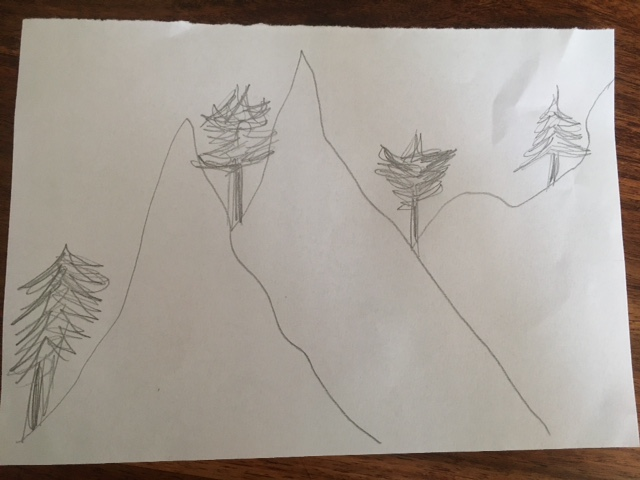
\includegraphics[width=0.25\linewidth]{images/croquis_3.jpg}
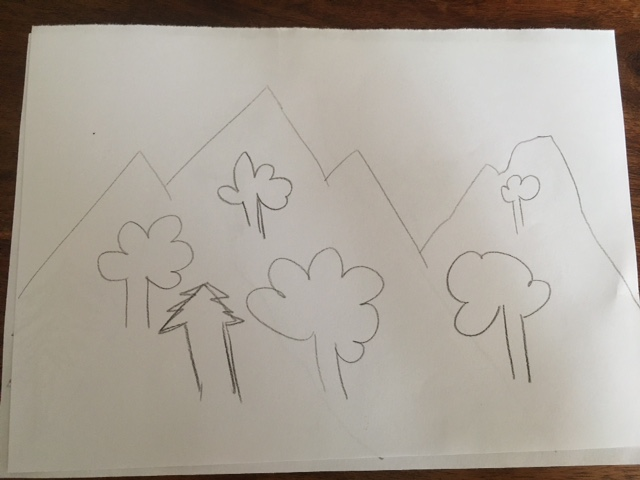
\includegraphics[width=0.25\linewidth]{images/croquis_4.jpg}
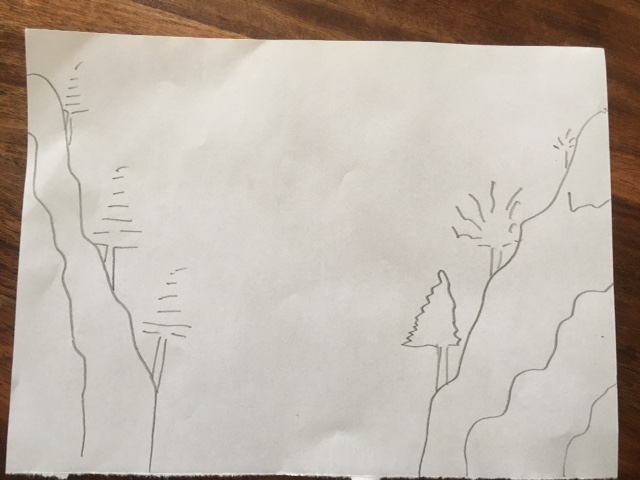
\includegraphics[width=0.25\linewidth]{images/croquis_5.jpg}
\paragraph{}


Nous pouvons dire que ce type de dessins constitue des "abstractions", que nous souhaitons convertir en peinture chinoises. En tant qu'humain nous percevons les objets de manière abstraite et sémantique.

Nous pouvons déjà noter qu'il n'existe pas une seule façon de représenter un paysage mais plusieurs. Selon le dessinateur, les dessins possèdent des niveaux "d'informations" plus ou moins élévé, c'est à dire plus ou moins "abstraits". La figure n°1 nous indique des arbres, mais nous ne savons rien de la forme potentiel que ceux-ci pourrais avoir (bien que nous pouvons dire qu'il s'agit plutôt d'un sapin que d'un pin). Tandis que sur la figure n°2 nous avons déjà plus de détails.



\chapter{Etat de l'art}
 
Nous présentons dans un premier temps l'architecture GANs, qui est au coeur de notre problématique. Nous présenterons également différents modèle existants sur lesquels nous avons testé nos données.

Enfin, nous évoquerons, de manière plus succincte, des recherches liées à notre sujet mais n'utilisant pas les réseaux de neurones afin de pouvoir identifier les avantages et inconvénients des deux mondes. 


\section{Généralité sur les GANs}

\paragraph{}
Les réseaux adverses génératifs sont une classe d'algorithmes d'apprentissage non-supervisé. Ces algorithmes ont été introduits dès 2014 par Goodfellow \cite{goodfellow2014generative} et permettent de générer des images avec un fort degré de réalisme. La structure des GANs se compose de deux parties, le générateur et le discriminateur. Le générateur génère des données et les soumets au discriminateur dont le but est d'évaluer le degré de crédibilité de la donnée. 


$G(z, 01)$ se charge de "mapper" le bruit $z$ vers l'espace désiré
$D(x, 02)$ retourne et la probabilité dans l'interval $[0,1]$ que $x$ vient du dataset original. Enfin $0i$ représente les poids définis par chacun des modèles.

Les poids sont donc mis à jours pour : 

1 - Maximiser la probabilité que les données $x$, soient classifiées comme appartenant au dataset d'origine. Soit maximiser la fonction de perte $D(x)$

2 - Minimiser la probabilité que de fausse images appartiennent au dataset d'origine. Soit minimiser la fonction de perte $D(G(z))$


Pour résumer c'est une sorte de jeu, dans lequel le générateur essai de maximiser la probabilité que sa sortie soit reconnu comme réel, tandis que le discriminateur essai de minimiser la même valeur.

Mathématiquement La fonction de perte peut-être écrite ainsi : 


\begin{center}
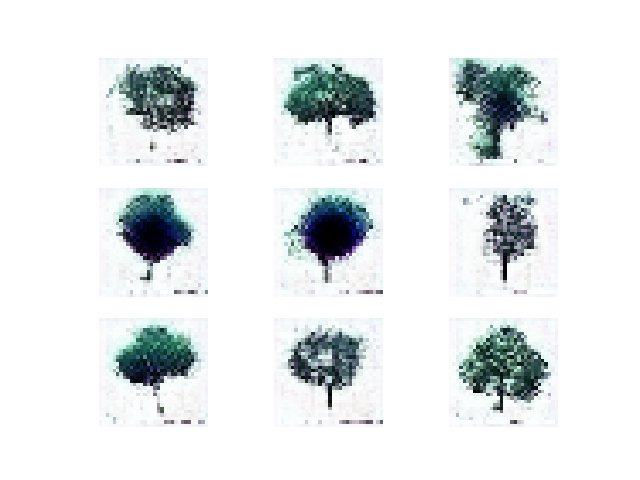
\includegraphics[scale=0.7]{images/tests_cgan.png}
\captionof{figure}{Test de génération d'arbres utilisant l'architecture DCGAN}
\label{fig1}
\end{center}

Les Gans conditionnels que nous abordons plus en détails plus loin, apprennent à partir d'une observation $x$ et d’un vecteur de bruit aléatoire $z$, vers $y$:$G:{x,z} →y$.

Il existe aujourd'hui une très grande variété de travaux de recherches implémentants les Gans (CGAN, Bayesian GAN, GYCLE GAN ...). Nous présentons ici des solutions existantes permettant de répondre partiellement à notre problématique.


\section{Génération d'image conditionnels}

Grâce aux conditionnals GANs il est aujourd'hui  possibles de générer des image réalistes basées sur des labels de classes, des textes ou des images.


\subsection{pix2pix}
Phillip Isola, Jun-Yan Zhu, Tinghui Zhou et Alexei A. Efros proposent en 2014 une nouvelle approche intitulée Image-to-Image Translation with Conditional Adversarial Networks.\cite{DBLP:journals/corr/GatysEB15a}
Leur contribution principale fut de montrer en quoi les cGans peuvent permettre de résoudre efficacement les problèmes de translation d'image et ainsi de proposer un framework pouvant être appliqué à n'importe quel domaine.

\subsection{GauGan}
Nvidia \cite{DBLP:journals/corr/abs-1903-07291} présente en 2019 une forme spécifique de génération d'image basé sur des "semantic segmentation mask". 

Selon les auteurs, les couches de normalizations ont tendance à faire perdre l' l'information contenu dans les masques sémantiques d'entrées car ils ne dépendent pas  de données externe. Ces derniers introduisent donc la notion de "normalization conditionnel" ou "adaptative", permettant notamment de prendre en compte les informations spatials.


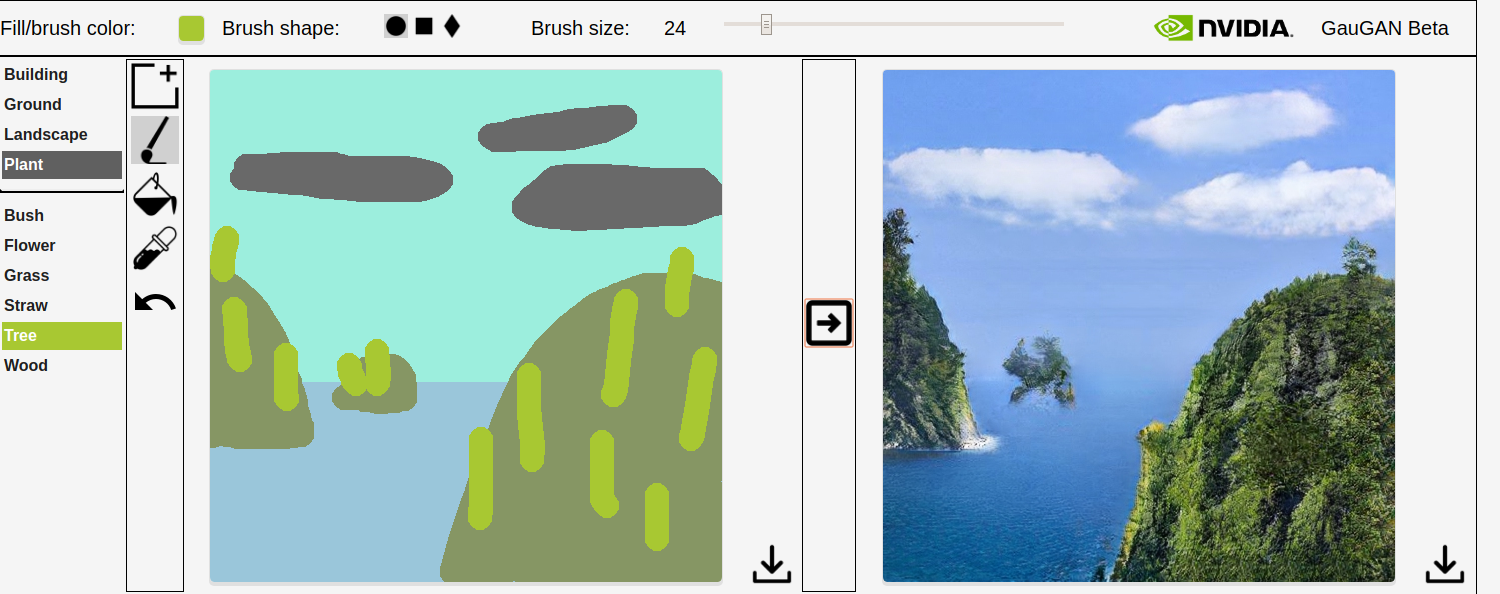
\includegraphics[width=1\linewidth]{images/test-gaugan.png}


\subsection{Le transfert de style neuronal}

Cette technique fut décrite par Leon A. Gatys dans son article "A Neural Algorithm of Artistic Style".~\cite{DBLP:journals/corr/GatysEB15a}

Celle-ci utilise trois images, la première est l'image d'entrée (bruit), la seconde représente le style de référence (comme une peinture par exemple), la dernière correspond à l'image que l'on souhaite transformer.

Le principe consiste à définir deux fonctions de distance. La première décrit comment le contenu de deux images sont différentes, et la seconde représente la différence de style. On obtient alors deux images, une pour le style souhaité, une pour le contenu.

L'objectif est de transformer l'image d'entrée en minimisant la distance avec l'image de contenu et avec l'image de style. On obtiens alors par rétropagation, une image qui correspond au contenu de l'image d'origine et au style souhaitée.

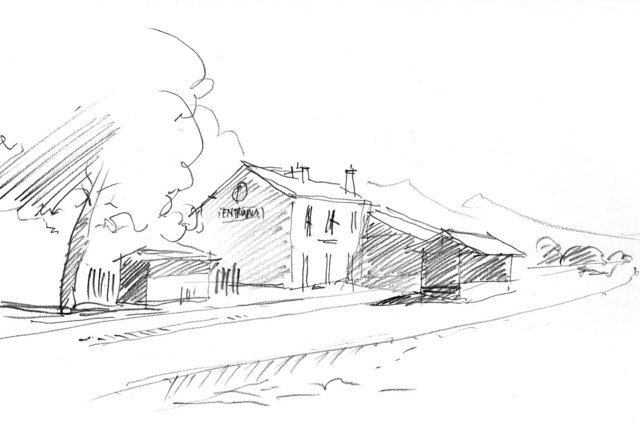
\includegraphics[width=0.5\linewidth]{images/transfert-style_1.jpg}
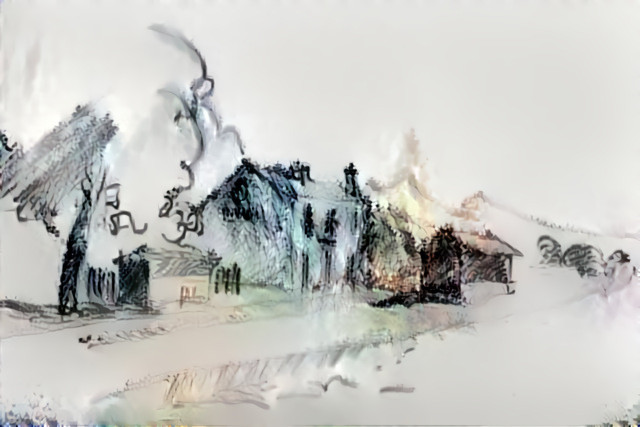
\includegraphics[width=0.5\linewidth]{images/transfert-style_2.jpg}
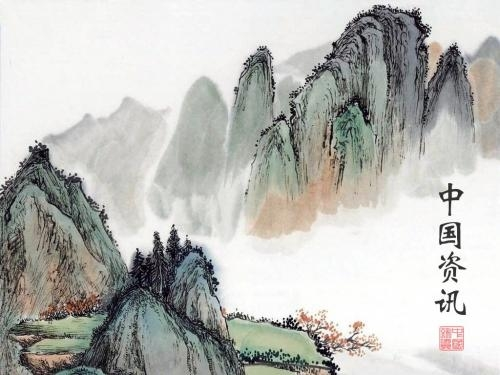
\includegraphics[width=0.5\linewidth]{images/transfert-style_3.jpg}

Cela nécessite la création d'un réseau convolutionnel, en effet le modèle doit être en mesure de capturer les invariances et de définir les caractéristiques de l'images (chats vs chien) afin d'en obtenir une compréhension générale.


L'avantage de cette technique est quelle nécessite pas de dataset à proprement parlé, seulement deux images en guise d'input



\subsection{Cycle Gan}

\subsection{Learning to Sketch}

Ce travail \cite{DBLP:journals/corr/abs-1805-00247} est important pour nous car il présente une méthode permettant de transformer une photos en croquis, en essayant d'imiter la façon de faire d'un humain. Leur model est capable de réaliser le croquis séquentiellement, c'est à dire ligne par ligne.
 
Les auteurs proposent de résoudre le problème "des styles subjectifs et variés de dessin humain" en utilisant un modèle hydride supervisé et non-supervisé. L'objectif étant de palier au "signal de supervision faible et bruyant" induit par l'écart important entre un croquis sa photo correspondante.

L'architecture est décomposé en 4 sous-modèle contenant chacuns leur propres sous-réseaux d'encodeurs et de décodeur : \\
- Une premier "supervisé" qui traduit une photo en croquis $D(E(photo))→sketch$ \\
- Un second supervisé aussi qui renvoie un croquis au domaine photo $(D(E(sketch))→photo)$ \\
- Un troisième non-supervisé pour reconstruire la photo $D(E(photo))→photo$
- Le dernier non-supervisé pour reconstruire le croquis $D(E(sketch))→sketch$

Le processus complet d'une photo vers un croquis serait donc : $x→Ep(x)→Ds(Ep(x))→Es(Ds(Ep(x))→Dp(Es(Ds(Ep(x)))$


\subsection{Photo-Sketching:Inferring Contour Drawings from Images}


"Les bords, les limites et les contours sont des sujets importants dans l’étude de la vision par ordinateur" \cite{DBLP:journals/corr/abs-1901-00542} 

L'article nous présente une technique pour générer un dessin de contour à partir d'une photo. Les Les "edges detector" traditionnels comme Canny, captent uniquement les signaux de haute fréquence dans l’image sans la comprendre. 

Les auteurs on collecté un dataset de 5000 pairs dessin/photos, créer la la plateform de crowdsourcing "Amazon Mechanical Turk". En effet aucun dataset de croquis actuellement connu ne répondait à la problématique (nombre d'éléments dans l'image, limites internes manquantes, le contenu non reconnaissable, les zones ombrées vides etc ..). Au final il s'agit d'un problème d'image-to-image translation. 

Un élément intéressant de ce modèle la possibilité d'avoir plusieurs labels différents pour la même image, car comme vu en ... Le même objet peut être interprété des plusieurs manière différentes. 


\subsection{Datasets disponibles}
Il est évident qu'il n'existe pas à l'heure actuel de dataset de paires croquis/peinture chinoise.

\subsubsection{Sketch}
Un des principaux problème de la recherche dans le domaine de la génération de croquis est le manque de dataset disponible. Aujourd'hui les plus grosses base de donnée que nous avons trouvé sont TU-Berlin \cite{eitz2012hdhso}, Sketchy \cite{sketchy2016} et Quickdraw. BSDS500

L'article (https://arxiv.org/pdf/1901.00542.pdf) est intéréssant car il nous offre une classification du niveau d'abstraction des croquis.
Un paramètre à prendre en compte également et le faite qu'il existe plus element dans le croquis.


Photo/croquis pair QMUL-Shoe-Chair-V2 dataset [46], qui contient plus de 8000 exemples.

\subsubsection{Peinture chinoises}
"La peinture chinoise désigne toute forme de peinture originaire de Chine ou pratiquée en Chine ou par des artistes chinois hors de Chine." \cite{} Il existe beaucoup de style courants et genres différentes (paysage, peinture narratives, faunes, flore, personnage). Nous avons aujourd'hui "scrapé" une collection de plus de 800 peintures.  noté qu'un des problèmes auquel nous allons faire face et la multiplicité des homothéties (Kakemono, paysage). Comme évoqué dans \cite{}, Les RCNN n'acceptent des images de tailles différents, il faudra donc trouver un moyen de trouver un bon compromis dans le redimensionnement de notre dataset.


\chapter{Propositions de solutions}

Voici les solutions envisagées  :

\section{Création du dataset en semi automatique}

En utilisant le logiciel LabelBox, il est possible de labeliser une image, en créant des sémantique layout[1]. Nous avons déjà un collection de plsu de 1000 images de peinture chinoises, les labelisés nous prendrait environ 2 jours hommes à raison d'une minute par image. Une fois cette étape réalisée, nous pourrions générer une ou plusieurs abstractions pour chaque peintures, en utilisant le dataset "quick draw" entre autres. Outre l'inconvénien du temps passé, cette solution n'est pas généralisable à autre chose que notre problématique.

\section{Photo-Sketching: Inferring Contour Drawings from Images}


\section{Abstraire une image via les CNN}
Nous savons qu'un CNN est capable de détecter des caractéristiques d'une image


Comme le prouve le travail de https://github.com/dribnet/perceptionengines, il est peut-être possible de générer un représentation abstraite en utilisant cette propriété des CNN.


\chapter{Conclusion et Perspectives\label{chap-conclusion}}

\bibliographystyle{alpha}
\bibliography{memoire}
\end{document}
